\section{実験装置}
実験装置を以下に示す.
アプローチするピーマンは前章でスキャンしたピーマンである.
\figref{Fig:finraymodel} \verb|〜| \figref{Fig:agristmodel} は作成したエンドエフェクタモデルである.
以降は, フィンレイエンドエフェクタを参考に作成したモデルをグリッパ型, 振動ナイフのエンドエフェクタを参考にしたものを振動ナイフ型, AGRISTのエンドエフェクタを参考にしたものを花柄アプローチ型と呼ぶ.
ピーマン株に対して各エンドエフェクタモデルを垂直にアプローチさせるための実験装置を \figref{Fig:device} に示す.


\vspace{5mm}
\begin{figure}[H]
     \centering
     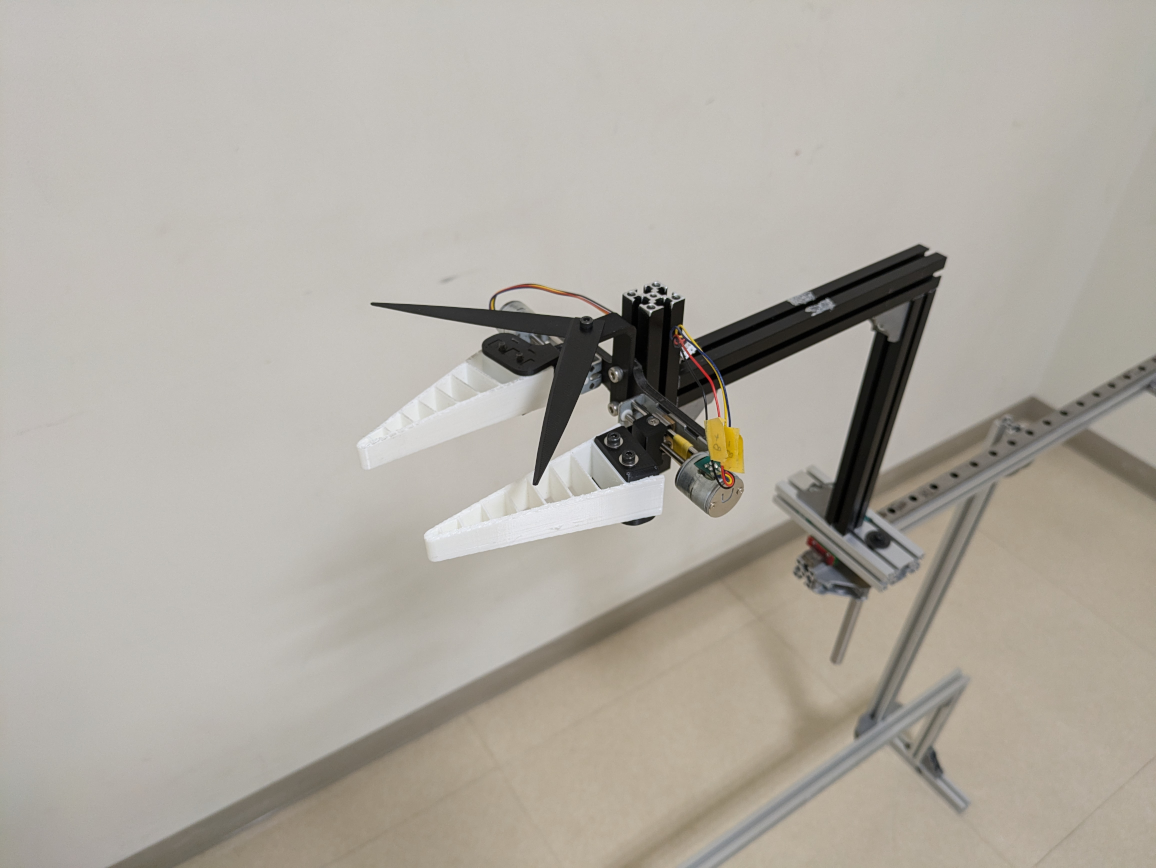
\includegraphics[width=100mm]{images/png/finray_model.png}
     \caption{End effector model① gripper type}
     \label{Fig:finraymodel}
   \end{figure}

\begin{figure}[H]
    \centering
    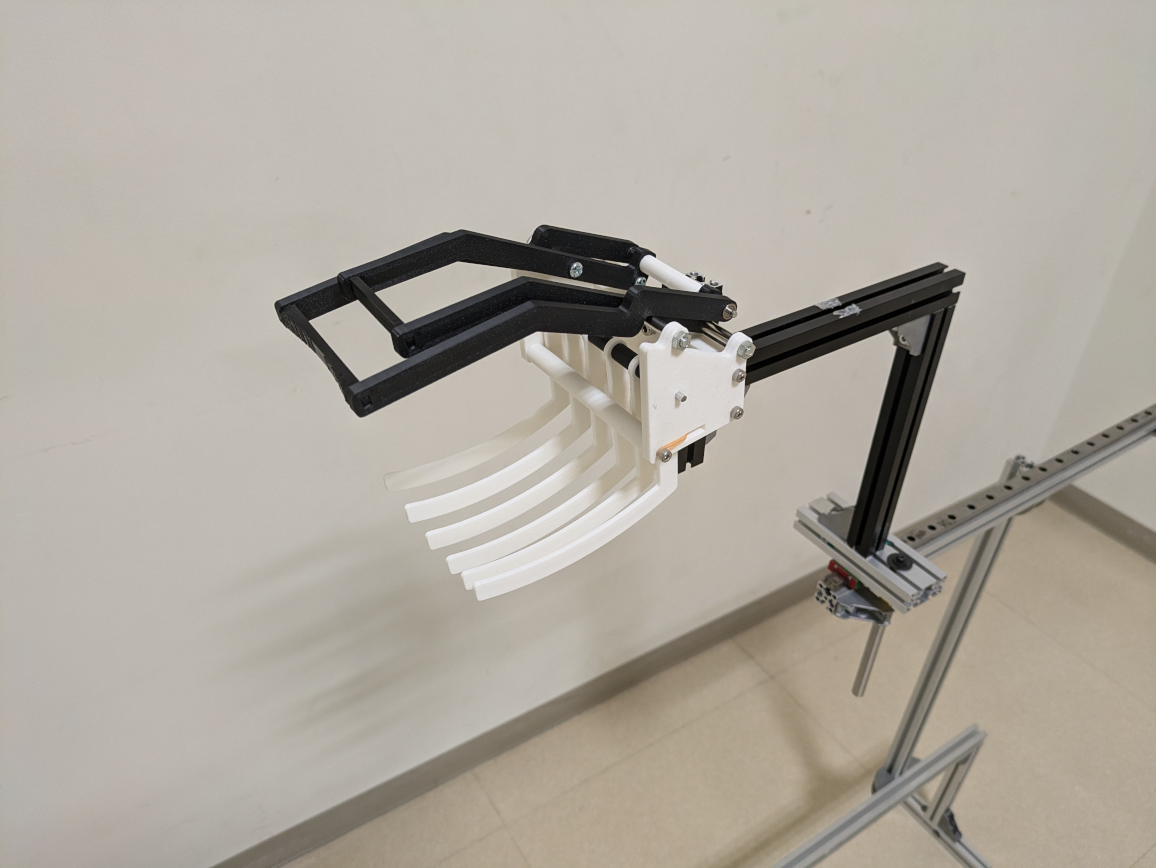
\includegraphics[width=100mm]{images/png/sweeper_model.png}
    \caption{End effector model② vibrating knife type}
    \label{Fig:sweepermodel}
   \end{figure}

\begin{figure}[H]
    \centering
    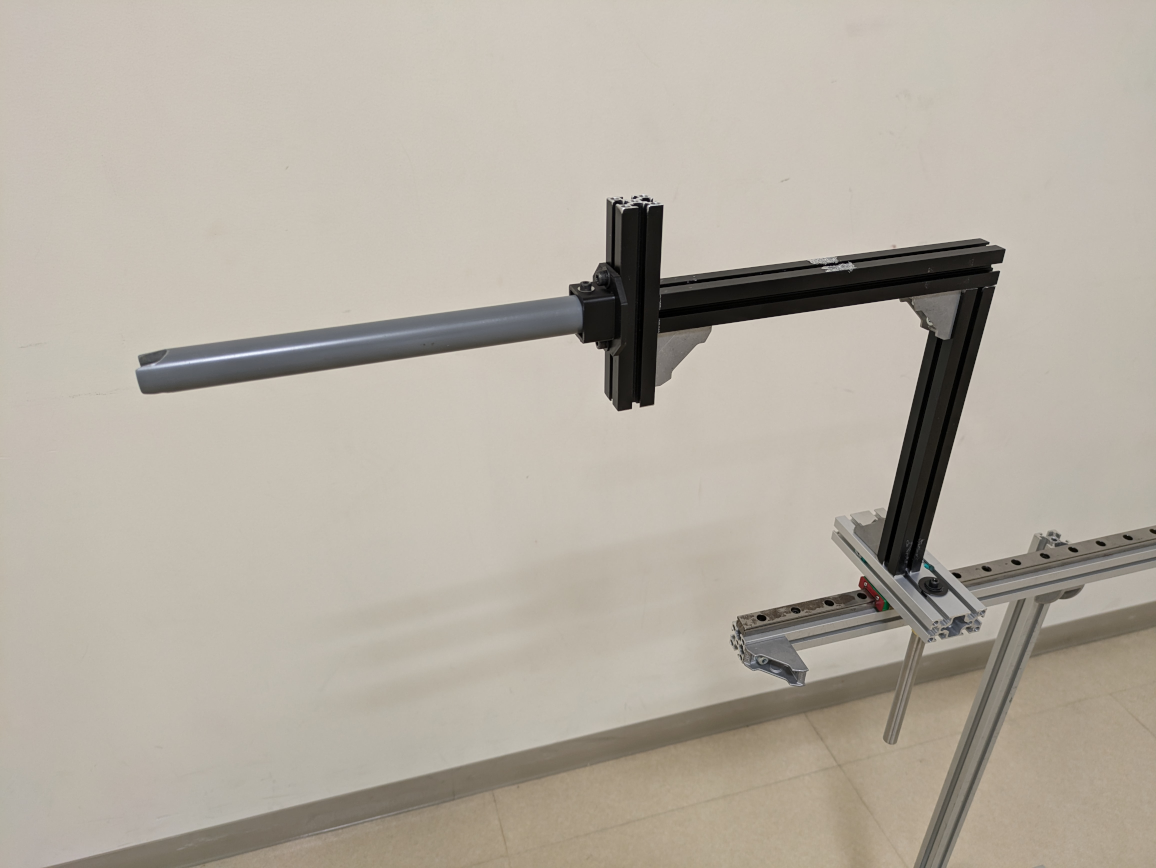
\includegraphics[width=100mm]{images/png/agrist_model.png}
    \caption{End effector model③ peduncle approach type}
    \label{Fig:agristmodel}
   \end{figure}

\begin{figure}[H]
    \centering
    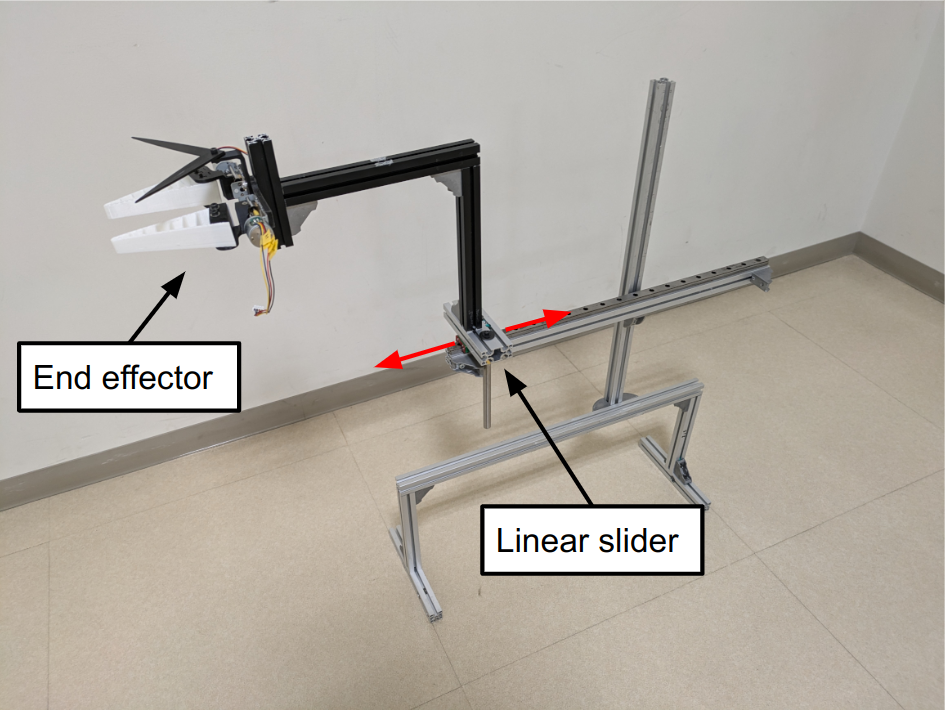
\includegraphics[width=100mm]{images/png/device.png}
    \caption{Experimental device}
    \label{Fig:device}
   \end{figure}
